\documentclass{beamer}
\mode<presentation>
\usepackage[utf8]{inputenc}
\usepackage{graphicx}
\usepackage[english,italian]{babel} % se non fosse inglese dovrei indicare la lingua nella quale sillabare [Italian]
%\usepackage{fancybox}
\useoutertheme{}
\usepackage{beamerthemeshadow}
\usepackage{ulem}
\usepackage{courier}
\usepackage{tikz}
\usepackage{listings}
\usepackage{amsfonts}
\usepackage{fontawesome5}
\usepackage{color,soul}
\usetikzlibrary{snakes}
%\usepackage{beamertexpower}
%\beamertemplatetransparentcovereddynamicmedium
\usetheme{GTER} %(se vuoi mettere l'autore)
\useinnertheme{rectangles}
%\useoutertheme{infolines}
\usecolortheme[RGB={151,215,0}]{structure}
%\usecolortheme[RGB={0,99,29}]{palette quaternary}

\setbeamercovered{transparent}
\setbeamerfont{frametitle}{size=\small,series=\bfseries}
\setbeamercolor{frametitle}{bg=gter!}

\definecolor{lightred}{rgb}{0.94,0.04,0.04}
\definecolor{aqua}{rgb}{0.00,0.80,1.00}
\definecolor{lightgreen}{rgb}{0.01,0.40,0.03}
\definecolor{limegreen}{rgb}{0.61,1.00,0.10}
\definecolor{peach}{rgb}{1.01,0.85,0.72}
\definecolor{purple}{rgb}{0.93,0.51,0.93}
\definecolor{indianyellow}{rgb}{0.98,0.75,0.30}
\definecolor{brick}{rgb}{0.70,0.13,0.13}
\definecolor{springsteen}{rgb}{0.00,0.49,0.19}
%%%%%%%%%%%%%%%%%%%%%%%%%%%%%%%%%%%%%%%%%%%%%%%%%%%%%%%%%%%%%%%%%%%%%%
% \definecolor{gter}{rgb}{0.00,0.49,0.22} %verde GTER estratto da gimp
\definecolor{gter}{RGB}{151,215,0}
%%%%%%%%%%%%%%%%%%%%%%%%%%%%%%%%%%%%%%%%%%%%%%%%%%%%%%%%%%%%%%%%%%%%%%
\definecolor{lightorange}{rgb}{1.01,0.50,0.00}
\definecolor{royalblue}{rgb}{0.25,0.41,1.00}
\definecolor{lightgray}{rgb}{0.94,0.94,0.94}

% \definecolor{links}{HTML}{2A1B81}
\hypersetup{colorlinks,linkcolor=lightgray,urlcolor=springsteen}

\title{Modulo 1 - QGIS}
\subtitle{Gestione del progetto}
\author[]{Gter srl Innovazione in Geomatica Gnss e Gis}
\author[]{Relatore: Simone Parmeggiani}
\date{Genova, Febbraio 2024} 
\logo{
\includegraphics[height=0.5 cm]{./Gter.png}}

\begin{document}
	{
		{
			\setbeamertemplate{footline}{} 
			\begin{frame}
				\titlepage
			\end{frame}
		}
		\addtocounter{framenumber}{-1}

\section{Introduzione}
\subsection{Introduzione}

\begin{frame}
   \frametitle{Progetto}

   Il menu Progetto fornisce le opzioni di accesso e di uscita del project files. Fornisce gli strumenti per:

   \begin{itemize}
            \item  Creare un Nuovo file da zero o utilizzando un altro file di progetto come modello
            \item Aprire un file di progetto, o apri da un GeoPackage, da un database PostgreSQL o Oracle
            \item Chiudere un progetto o riportalo al suo ultimo salvataggio
            \item Salva un progetto in formato .qgs o .qgz, sia come file che all’interno di un database GeoPackage, PostgreSQL o Oracle.
    \end{itemize}       
\end{frame}

\begin{frame}
   \frametitle{Progetto - Layer mancanti}

   Qualora un layer precedentemente caricato sul progetto venisse cancellato o spostato di percorso, una finestra ci avvertirà del mancato caricamento, fornendo una funzionalità per gestire l'incongruenza

    \begin{figure}[h]
        \centering
        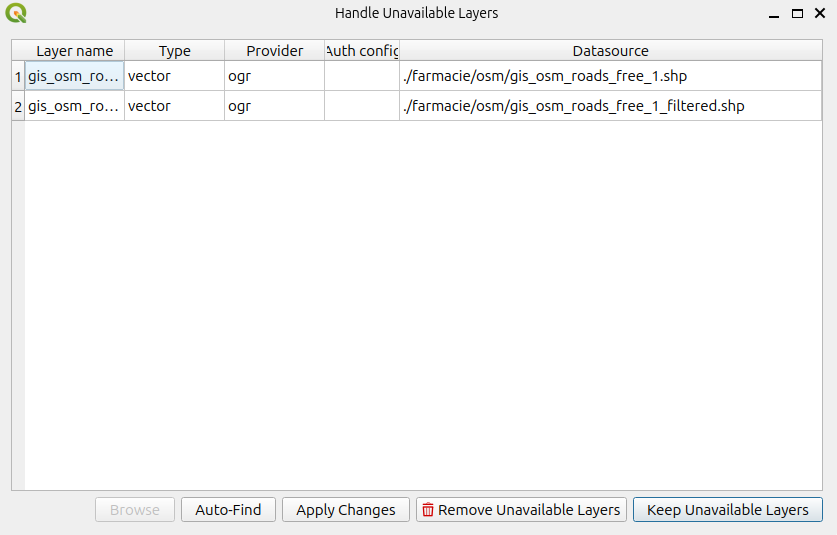
\includegraphics[width=0.3\textwidth]{corso2023/progetto.png}
    \end{figure}     
\end{frame}

\begin{frame}
   \frametitle{File Vettoriali}
   \begin{itemize}
            \item  I dati vettoriali sono usati per rappresentare gli oggetti del mondo reale in un GIS.
            \item Un oggetto vettoriale può avere una geometria di tipo punto, linea o poligono.
            \item Ogni geometria vettore contiene dati di attributo che lo descrivono, una tabella degli attributi
            \item La geometria dell’elemento è definita in termini di vertici.
             \end{itemize}       
\end{frame}


\begin{frame}
  \frametitle{Modello vettore}
  \begin{columns}
		\begin{column} {0.75\textwidth}	
			Il modello vettoriale indica una rappresentazione di entità geografiche attraverso: 
   	 \begin{itemize}
   		\item punti,
   		\item linee,
   		\item poligoni.
   	\end{itemize}
  		I modelli vettoriali sono particolarmente utili per rappresentare e memorizzare oggetti discreti come edifici, strade, particelle, etc.					
		\end{column}
		\begin{column} {0.25\textwidth}	
			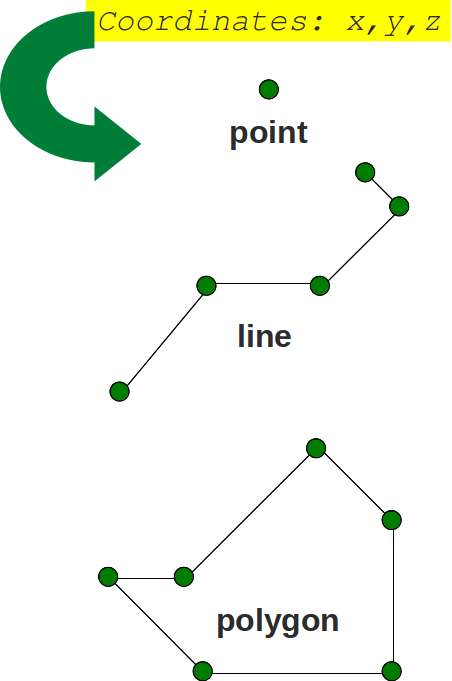
\includegraphics[width=1\textwidth] {./digitizing_pics/geom2.png}	
		\end{column}
	\end{columns}
   
  \begin{center}
  		\textbf{Nel modello vettoriale le informazioni su oggetti discreti sono codificate ed archiviate come insieme di coordinate x,y,z}.
  \end{center}    
\end{frame} 

\begin{frame}
  \frametitle{Modello vettore}
 \begin{itemize}
    \item Punti
    \begin{figure}[h]
        \centering
        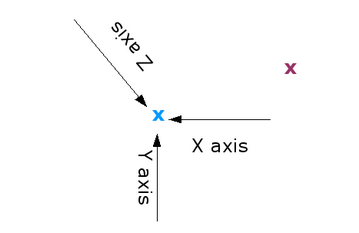
\includegraphics[width=0.3\textwidth]{corso2023/punto.png} % Sostituisci con il nome del tuo file immagine
    \end{figure}

    \item Polilinee
    \begin{figure}[h]
        \centering
        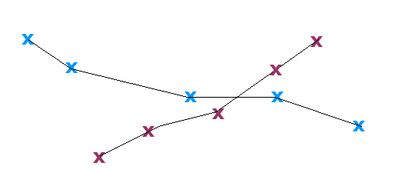
\includegraphics[width=0.3\textwidth]{corso2023/polilinea.png} % Sostituisci con il nome del tuo file immagine
    \end{figure}

    \item Poligoni
    \begin{figure}[h]
        \centering
        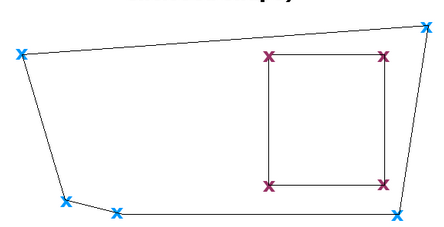
\includegraphics[width=0.3\textwidth]{corso2023/poligono.png} % Sostituisci con il nome del tuo file immagine
    \end{figure}
\end{itemize}

\end{frame} 

\subsection{File raster}
\begin{frame}
  \frametitle{Modello raster }
   Preparare e caricare le immagini satellitari su QGIS. Carica questo file raster in QGIS facendo click su \textbf{Layer} $\rightarrow$ \textbf{Add Raster Layer}.
		    \begin{center}
			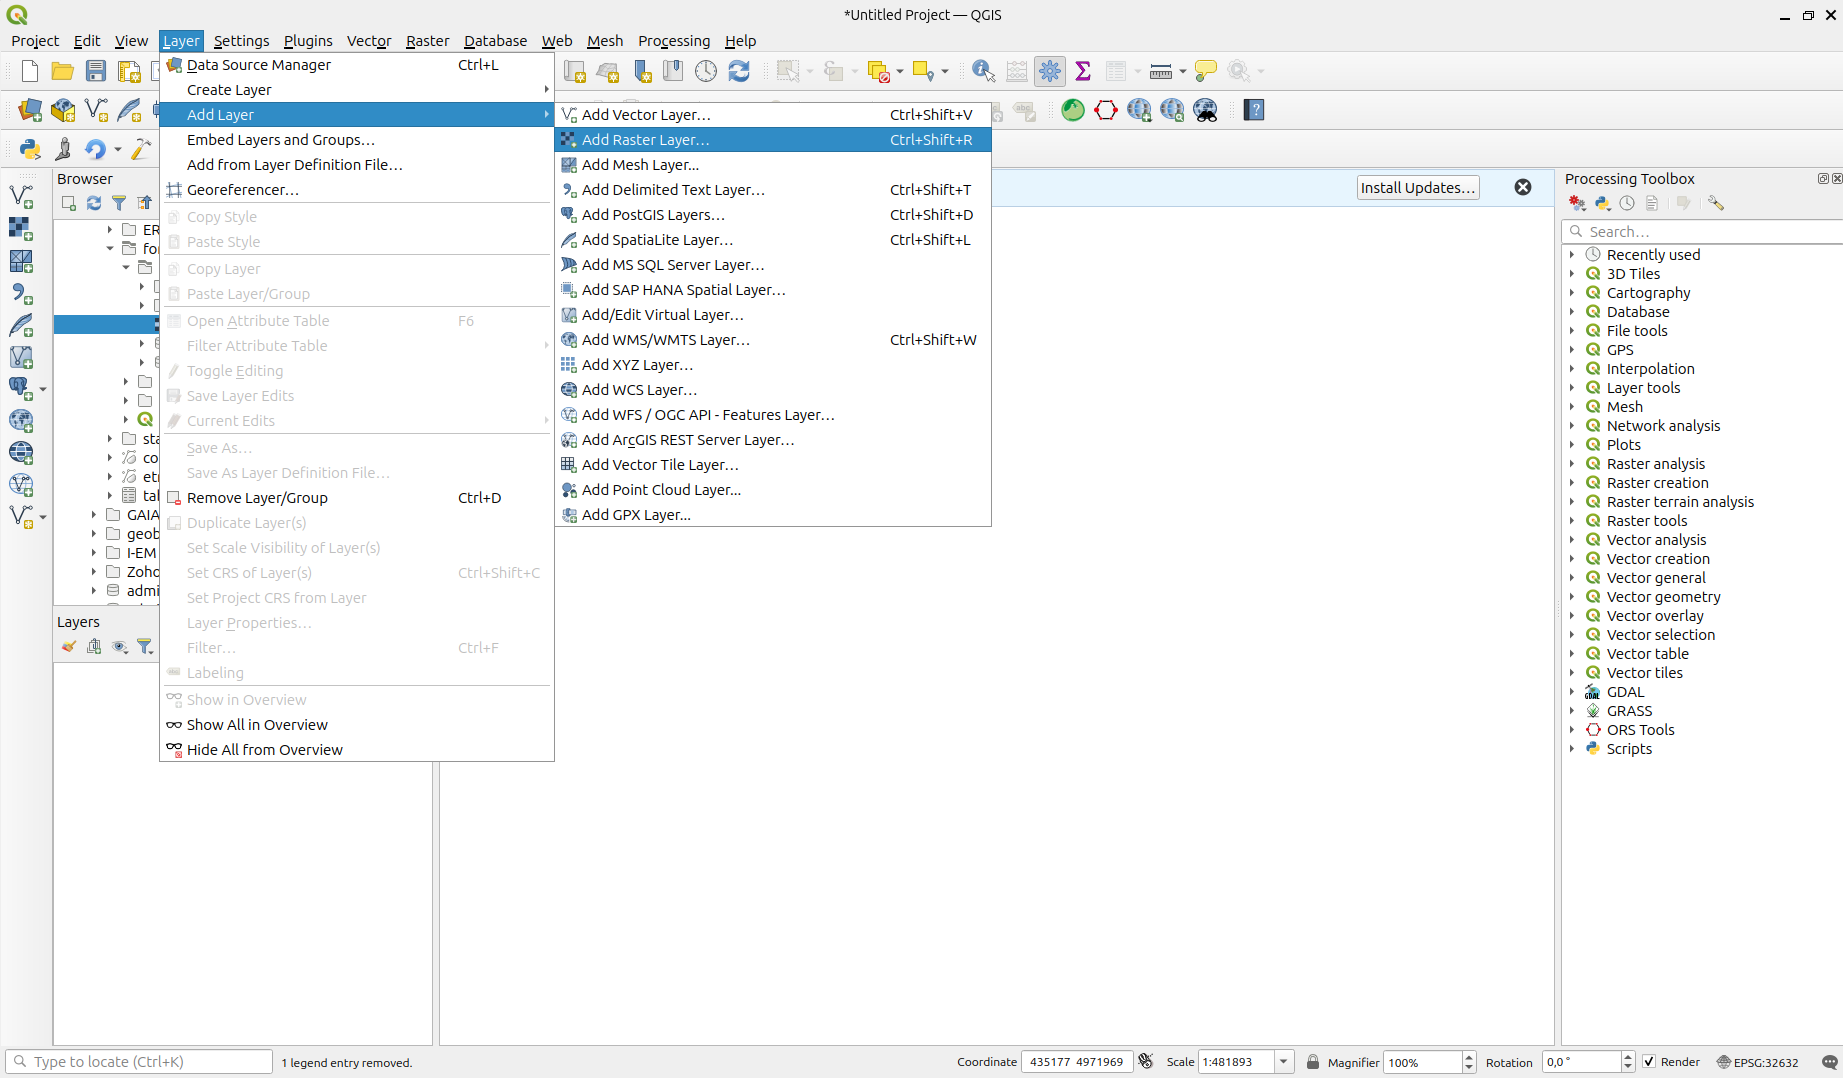
\includegraphics[width=0.80\textwidth] {digitizing_pics/add_raster.png}
		    \end{center}
\end{frame} 


\begin{frame}
  \frametitle{Visualizzare raster scala di grigi}
    Se il file raster contiene una sola banda, di default verrà rappresentato in scala di grigi
		    \begin{center}
			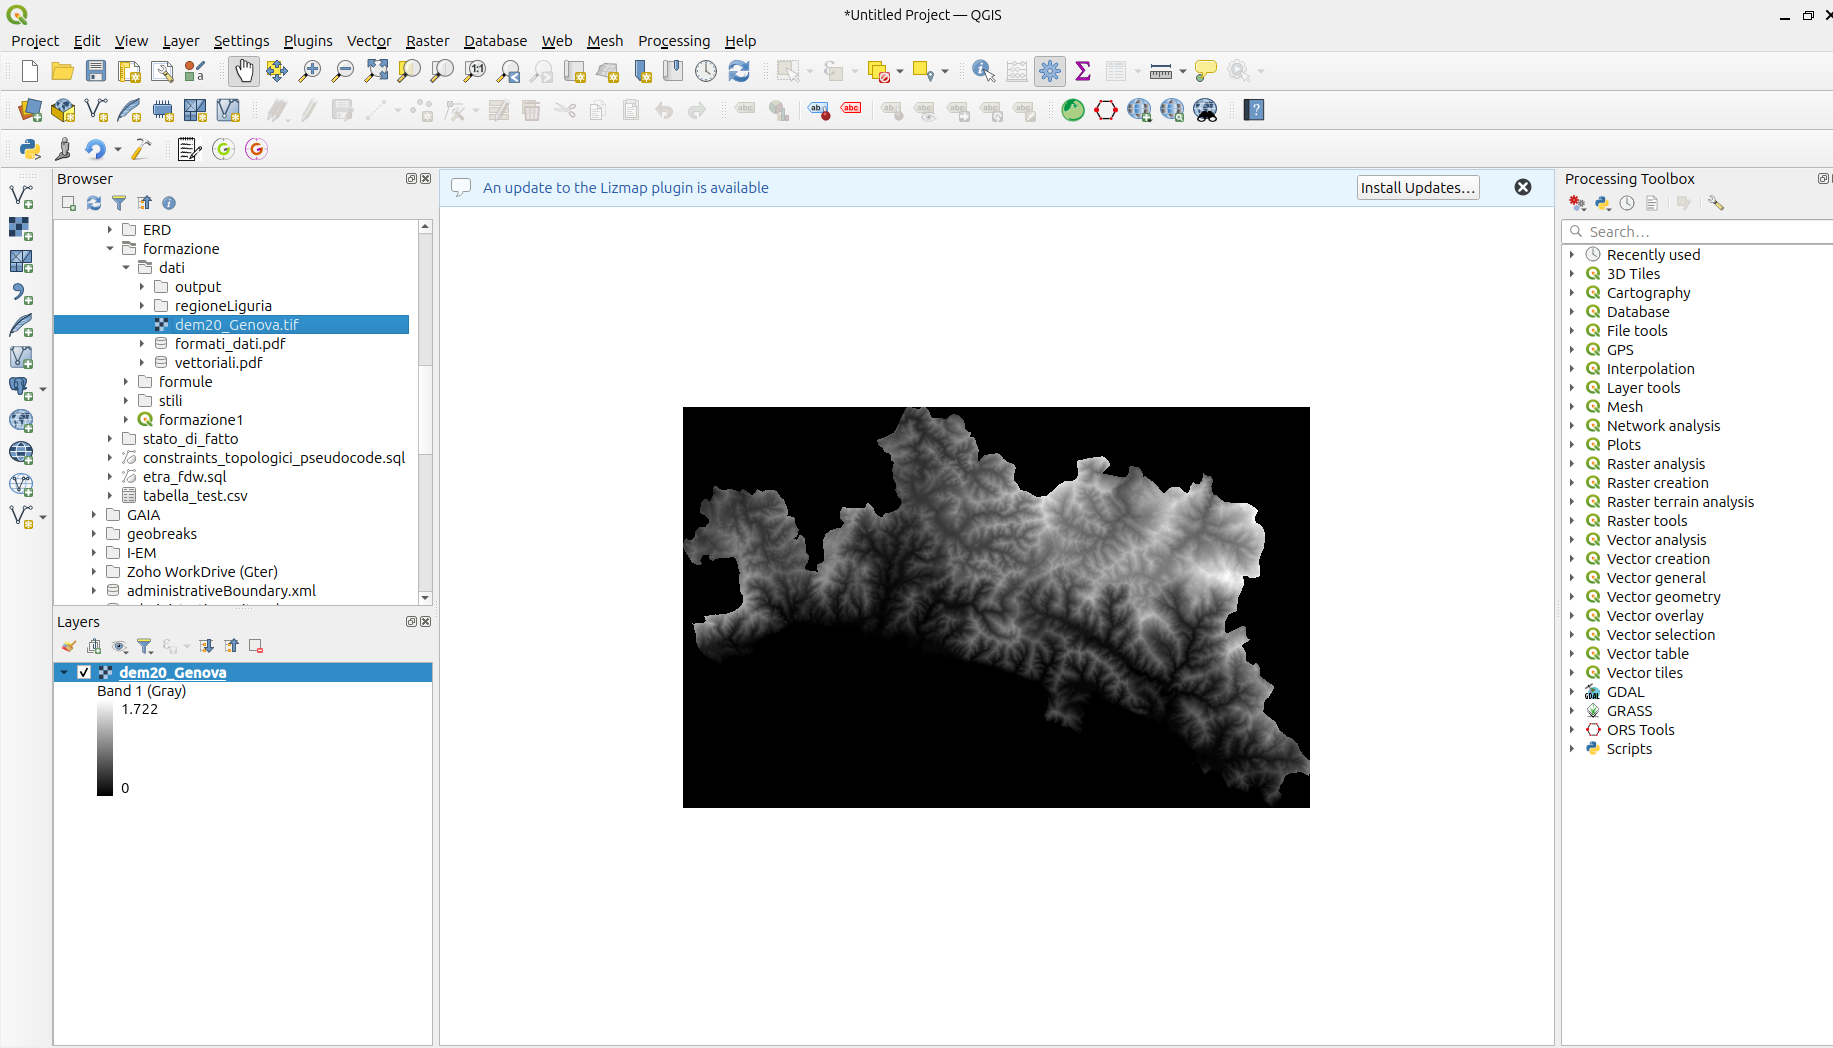
\includegraphics[width=0.90\textwidth] {digitizing_pics/grey.png}
		    \end{center}
\end{frame} 


\begin{frame}
  \frametitle{Visualizzazione personalizzata tramite categorie}
    E' possibile tuttavia modificare le impostazione di visualizzazione \textbf{Click dx sul Layer} $\rightarrow$ \textbf{Properties} $\rightarrow$ \textbf{Symbology} $\rightarrow$ \textbf{Render type = Singleband pseudocolor} e settare range e colori di visualizzazione.
		    \begin{center}
			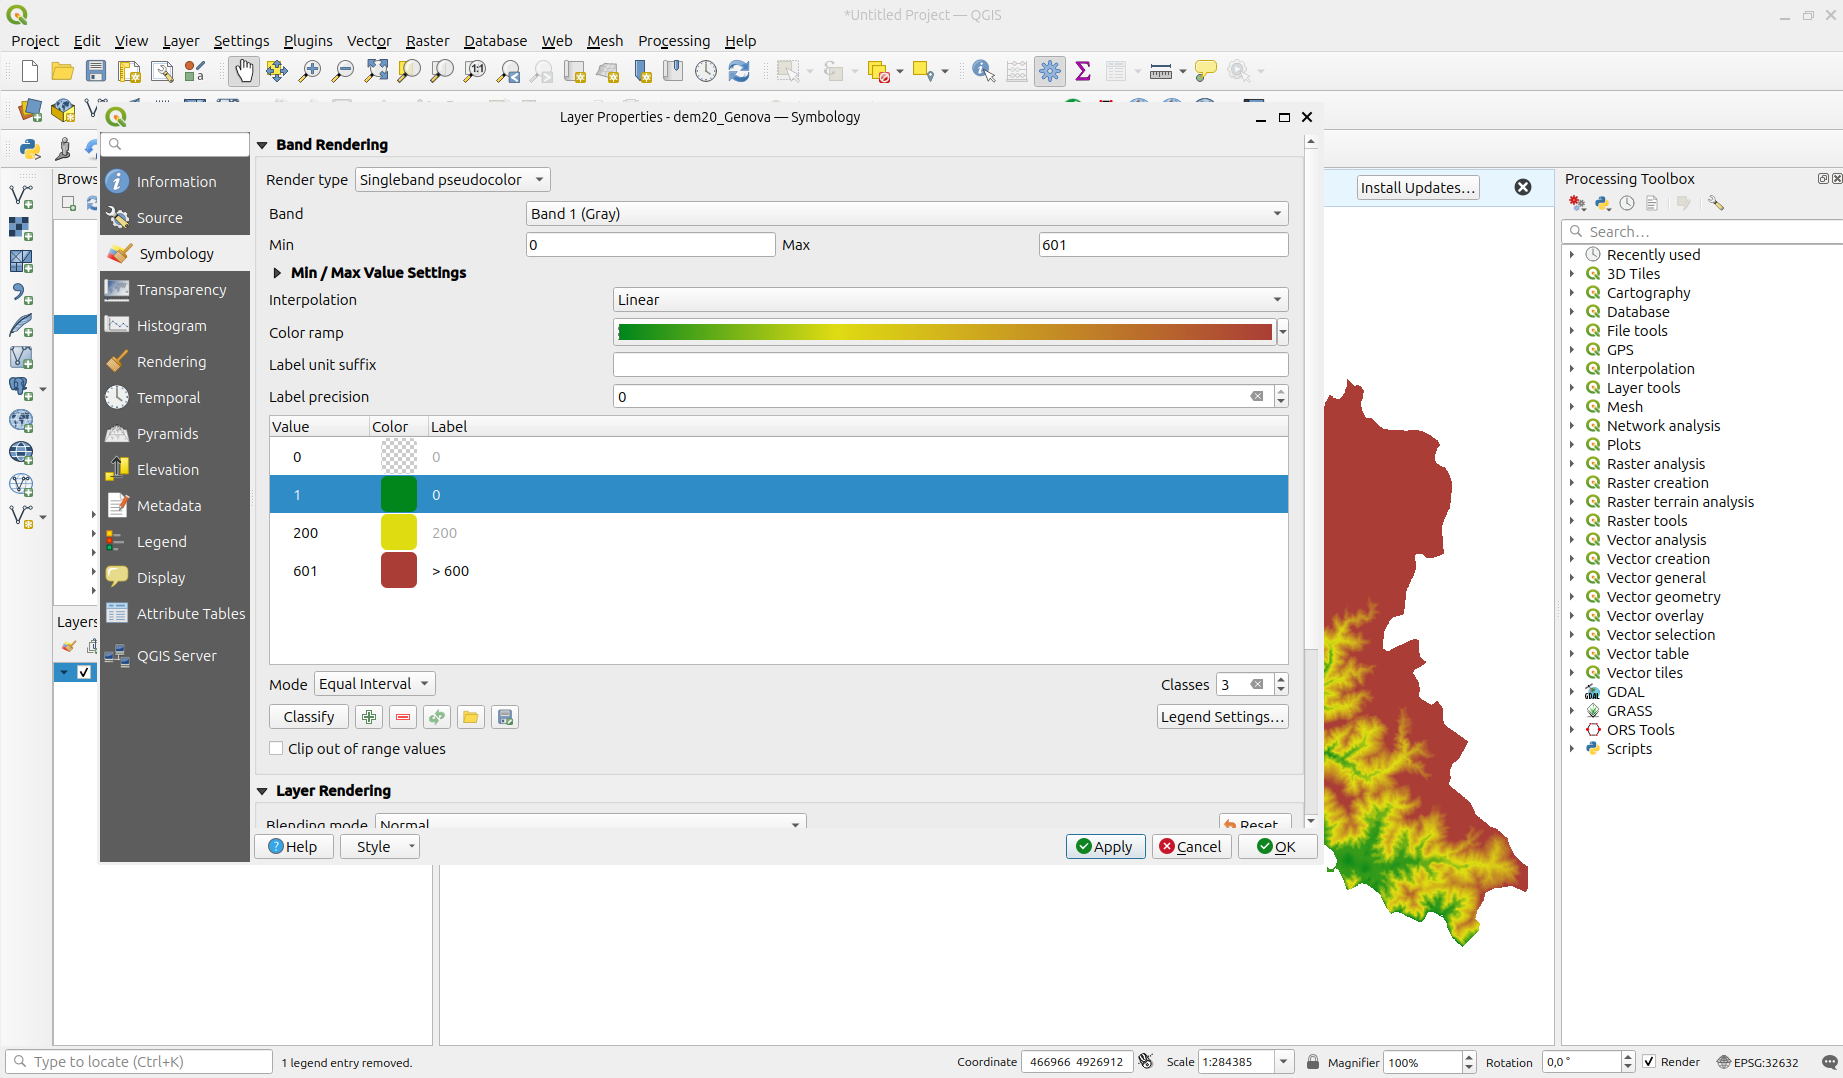
\includegraphics[width=0.90\textwidth] {digitizing_pics/categories.png}
		    \end{center}
\end{frame}

\begin{frame}
  \frametitle{Visualizzazione personalizzata tramite categorie}

		    \begin{center}
			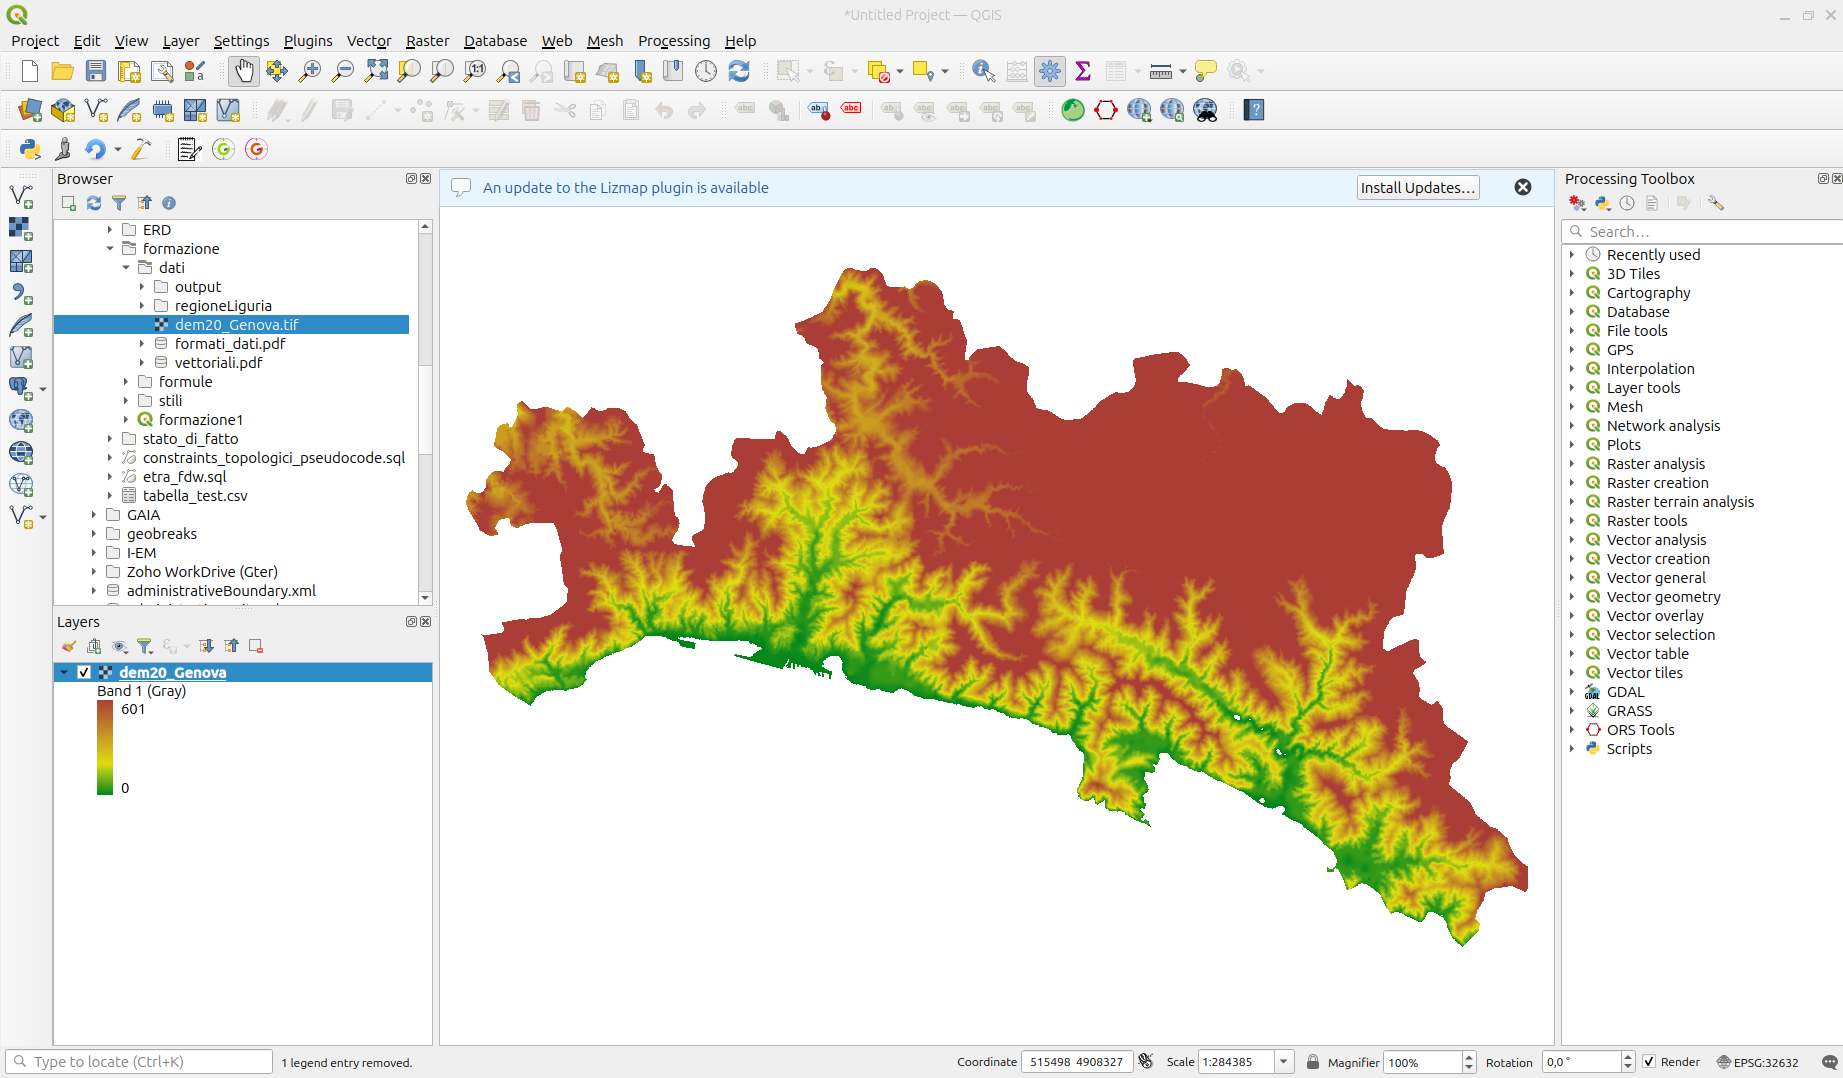
\includegraphics[width=0.90\textwidth] {digitizing_pics/categories2.png}
		    \end{center}
\end{frame} 


\section{Editing}

\subsection{Elementi di Base: Creazione nuovo layer vettoriale}

\begin{frame}
    \frametitle{Creazione di nuovo file: formati file vettoriali}
    \begin{center}
        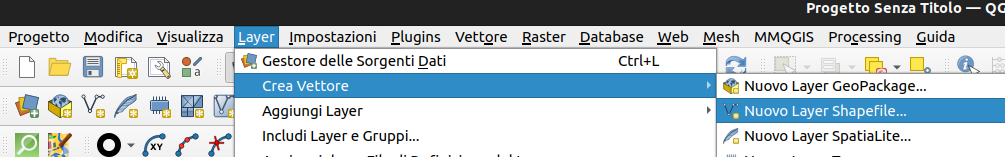
\includegraphics[width=1\textwidth]{corso2023/editor.png}
    \end{center}
    
    \begin{columns}
        \begin{column}{0.5\textwidth}
            Sono formati di uso comune:
            \begin{itemize}
                \item SHP (ESRI shapefile)
                \item Geopackage
                \item DB (es. postgress postgis \& spatial lite)
                \item CSV
                \item DXF (interoperabilità con CAD)
            \end{itemize}
        \end{column}
    \end{columns}
\end{frame}

 \begin{frame}
   \frametitle{Creazione di nuovo layer vettoriale}
   Proviamo a creare ad esempio un nuovo shapefile:
 	\begin{columns}
		\begin{column} {0.5\textwidth}	
			 \begin{center}
			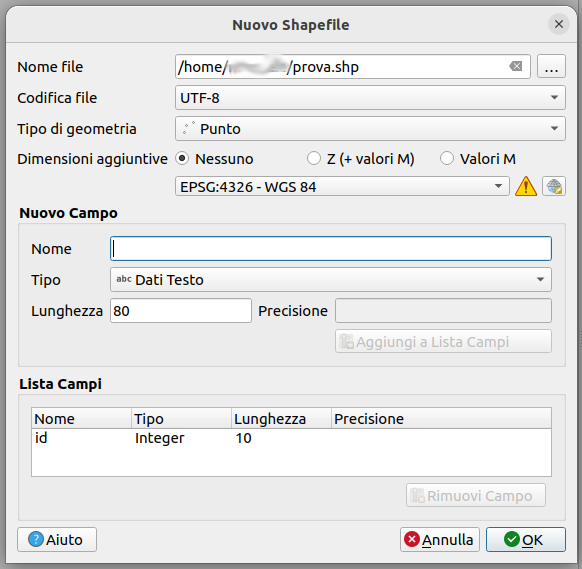
\includegraphics[width=1\textwidth] {digitizing_pics/Nuovo Layer Vettoriale 2022-10-11 09-59-20.png}
		    \end{center}
		\end{column}
 
		\begin{column} {0.5\textwidth}	
    	 \begin{itemize}
    		\item la tipologia geometrica (punti, linee o poligoni)
    		\item SR (Sistema di riferimento),
    		\item tabella degli attributi (specificare nome e tipologia dei vari campi della tabella associata)
    	\end{itemize}				
		\end{column}
		
	\end{columns}	
	   
\end{frame} 

\begin{frame}
    \frametitle{Scelta del SR}
    La selezione del SR associato al nuovo layer può essere fatta attraverso i codici     \href{http://www.epsg.org/}{\textcolor{gter}{\emph{EPSG}}} che li identificano in modo univoco.
    \begin{center}
        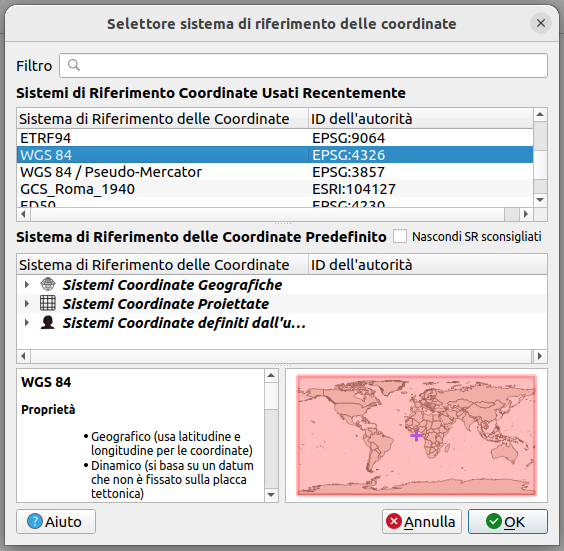
\includegraphics[height=.75\textheight] {digitizing_pics/Scelta SR.png}
    \end{center}
\end{frame} 


\begin{frame}
   \frametitle{Creazione di nuovo layer vettoriale}
 	\begin{columns}
		\begin{column} {1\textwidth}	
			 \begin{center}
			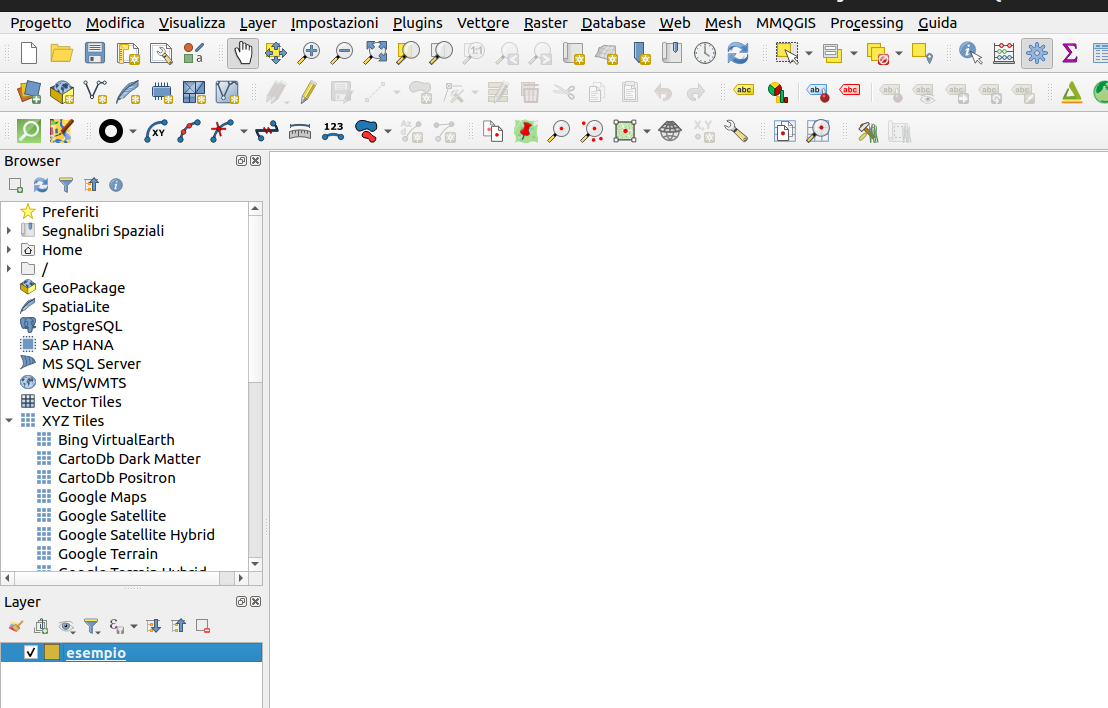
\includegraphics[width=1\textwidth] {corso2023/esempio poligono.png}
		    \end{center}
		\end{column}
 		
	\end{columns}	
	   
\end{frame}

\begin{frame}
\frametitle{Creazione di nuovo layer vettoriale}
 \begin{itemize}
    		\item La tabella attributi è una componente chiave di un dataset geospaziale. Contiene informazioni alfanumeriche relative alle entità spaziali sulla mappa, come punti, linee e poligoni. Questi dati aggiungono dettagli sulle caratteristiche delle feature geospaziali e consentono agli utenti di associare informazioni non spaziali alle posizioni geografiche, rendendo possibile l'esecuzione di interrogazioni, analisi e visualizzazioni basate su tali dati.
    		
    		\item La creazione della tabella degli attributi può avvenire concomitantemente alla creazione del vettore, permettendo successivamente di apportare ulteriori perfezionamenti. In alternativa, è contemplata la possibilità di raffinire l'oggetto vettoriale in un momento successivo attraverso un aggiornamento.
    	\end{itemize}		
\end{frame} 

\begin{frame}
\frametitle{Creazione di nuovo layer vettoriale}
\begin{itemize}
\item Per accedere alla tabella attributi di un vettore bisogna usare il pulsante destro del mouse, sul vettore nel menù layer, cliccare la voce  tabella attributi
\end{itemize}
\begin{center}
		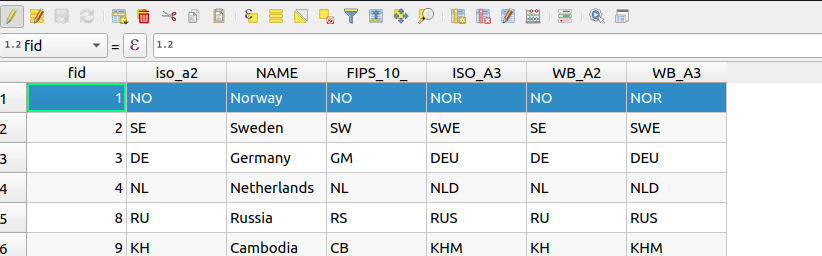
\includegraphics[width=1\textwidth] {corso2023/tab1.png}
	\end{center}
\end{frame} 


\begin{frame}
   \frametitle{Considerazioni e consigli utili}

    \begin{itemize}
	    \item Fino a quando non si salva è sempre possibile annullare le operazioni precedenti una a una (undo).
	    \item Un buon consiglio è comunque quello di salvare le operazioni di editing andate a buon fine per evitare di perdere del lavoro!
	    \item Al termine dell'editing viene richiesto se salvare o meno. Non salvando tutte le modifiche effettuate dopo l'ultimo salvataggio verranno automaticamente annullate. 
    \end{itemize}
\end{frame}

\section{Editing attributi}

\subsection{Query}

\begin{frame}
   \frametitle{Sfruttiamo una parte della Potenza dei GIS: Le interrogazioni}
   La tabella degli attributi consente la gestione dei dati alfanumerici associati alle geometrie. Attraverso la tabella degli attributi è possibile effettuare ricerche e selezionare record in base ai valori in essa contenuti.\\ATTENZIONE: è importante notare che alcune operazioni, come la selezione o l'eliminazione, incidono anche sulle geometrie associate. 
		    \begin{center}
			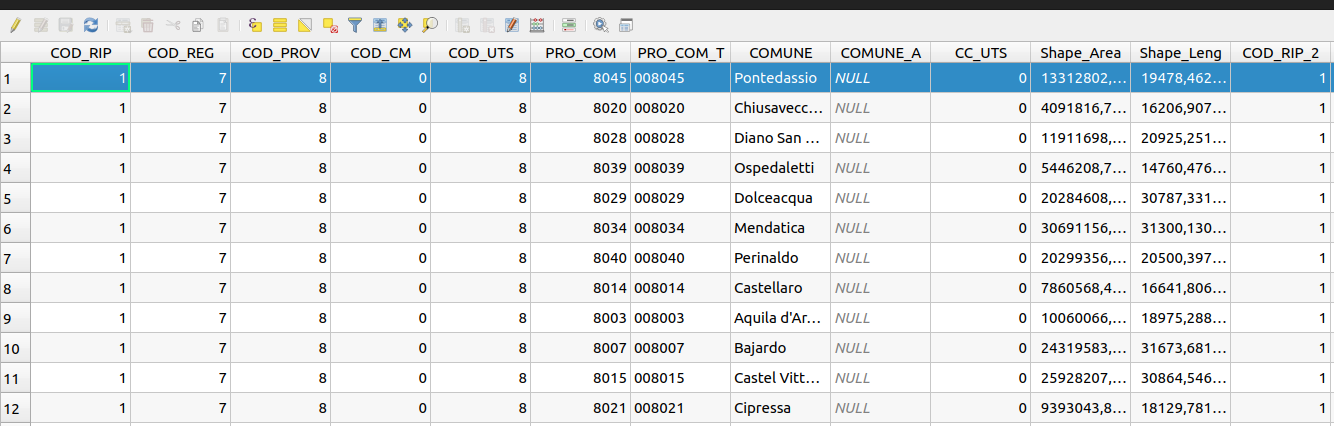
\includegraphics[width=0.70\textwidth] {corso2023/liguria1.png}
		    \end{center}
\end{frame}

\begin{frame}
   \frametitle{Sfruttiamo una parte della Potenza dei GIS: Barra della tabella attributi}
   \begin{figure}
       \centering
       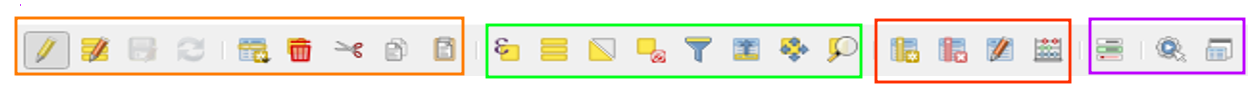
\includegraphics[width=1\linewidth]{Screenshot_2023_10_14-1.png}
       \begin{itemize}
          \begin{itemize}
  \item {\color{orange} Comandi di editing}
  \item {\color{green} Comandi di Zoom, Selezione, Filtro}
  \item {\color{red} Comandi di modifica della struttura della tabella. A tal proposito si veda anche lo strumento Riorganizza campi da Processing}
  \item {\color{magenta} Comandi azione e aggancio finestra}
\end{itemize}
            
           
           
       \end{itemize}
       
   \end{figure}
  
\end{frame}


 \begin{frame}
   \frametitle{Estrzione dei dati}
  Supponiamo di voler ottenere dalla tabella attributi tutti i Comuni che ricadono nella provincia di Savona per farlo possiamo usare lo strumento selezione per espressione, presente nel menù tabella attributi
  \begin{figure}
      \centering
      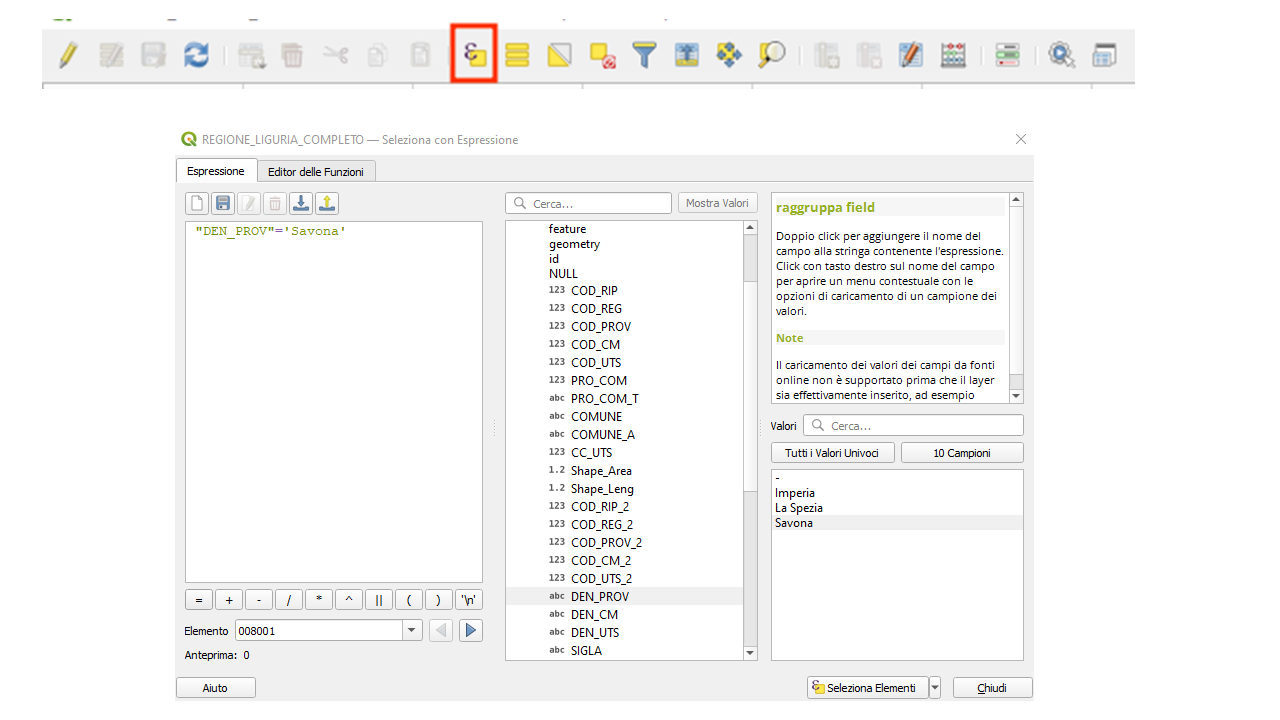
\includegraphics[width=0.7\linewidth]{Diapositiva1.PNG}
      
      
  \end{figure}

 
		
    %In the query builder window \textbf{Fields}, \textbf{Values}, \textbf{Operators} and \textbf{SQL where clauses} are shown. In this particular example, we want to highlight the museums (musei) of the town of Genova. We select: \tiny{COMUNE Fields = Genova} and click OK.
		    
\end{frame}



 \begin{frame}
   \frametitle{Risultato dell'estrazione dati}
   Il risultato dello strumento selezione per espressione evidenzia tutti i Comuni che ricadono nella Provincia di Savona sia nella tabella che su mappa.
   \begin{figure}
       \centering
       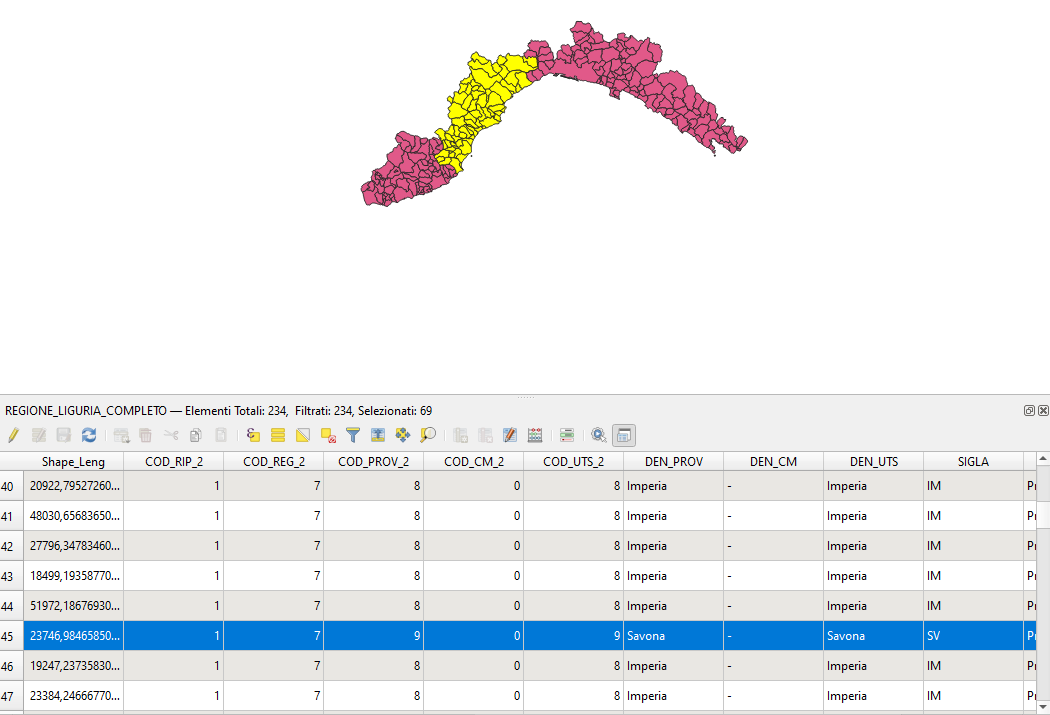
\includegraphics[width=0.8\linewidth]{savona.png}
       
       
   \end{figure}
		    
\end{frame}

 \begin{frame}
   \frametitle{Usiamo la selezione per modificare dei dati}
   Supponiamo che il Comune di Tiglietto (GE) sia passato alla provincia di Savona, ciò che cambia è solamente l'attributo dunque procediamo all'editing modificando la denominazione della provincia di Tiglietto, facendo uso dello strumento Filtro/Selezione
   \begin{itemize}
       \item Contestualmente alla modifica degli attributi, QGIS consente anche la possibilità di modificare la geometria relativa a Tiglietto
   \end{itemize}
   \begin{figure}
       \centering
       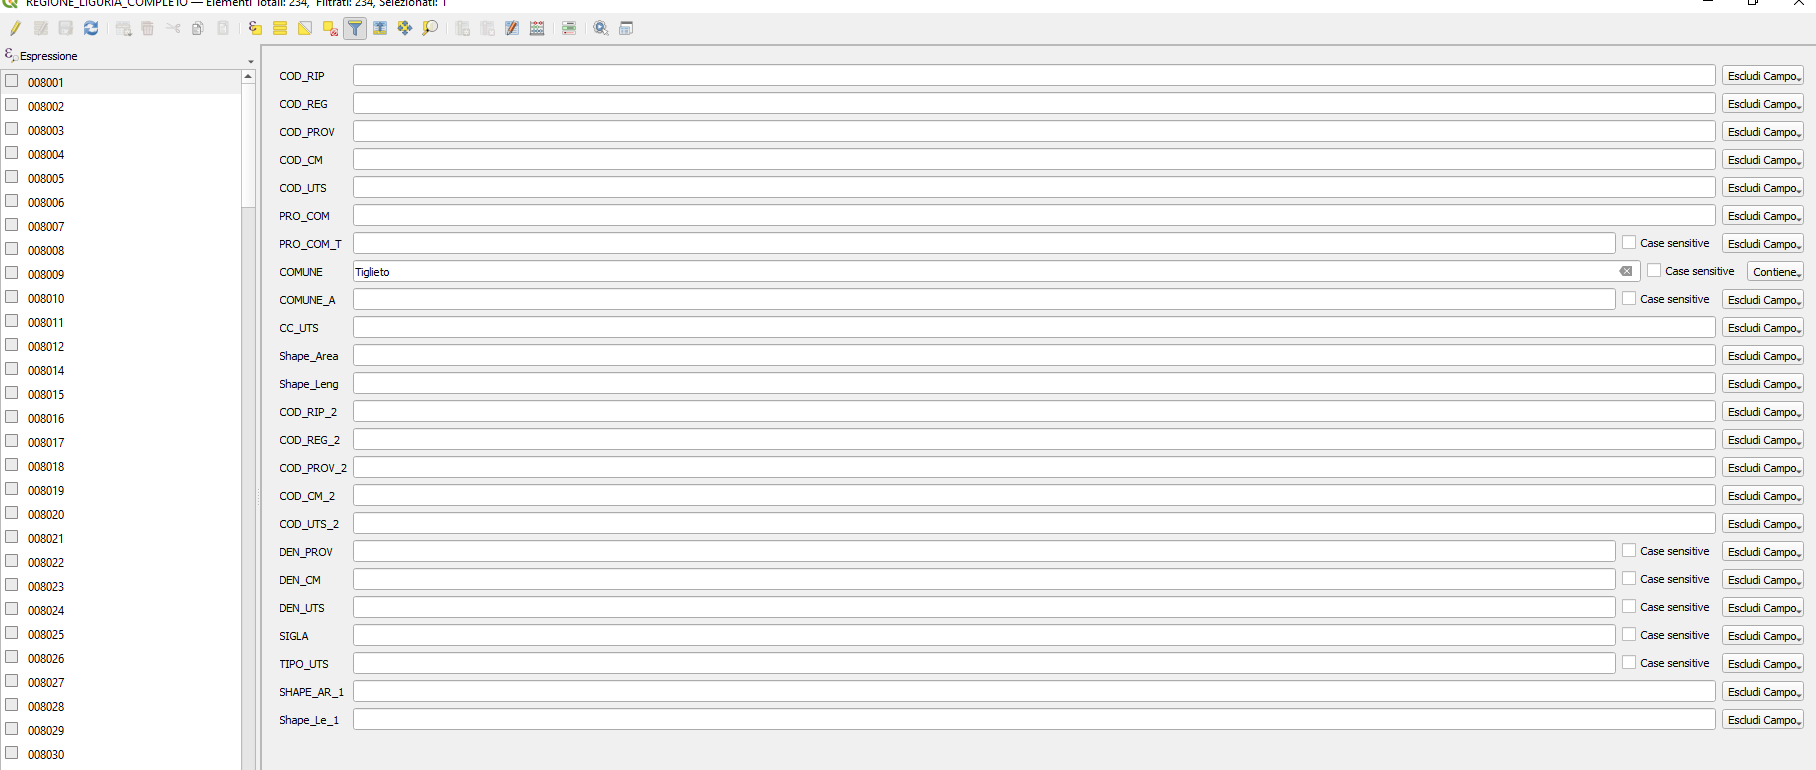
\includegraphics[width=0.75\linewidth]{tiglietto.png}
       
       
   \end{figure}
		    
\end{frame}


\begin{frame}
   \frametitle{Usiamo la selezione per modificare dei dati}
   \begin{figure}
       \centering
        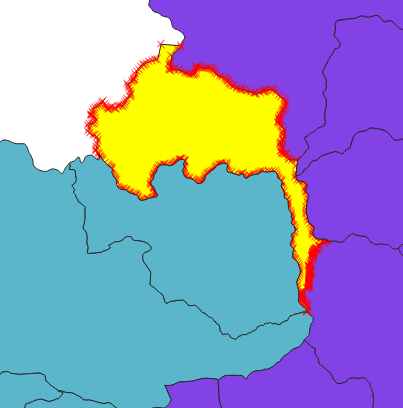
\includegraphics[width=0.5\linewidth]{tiglietto2.png}
        
   \end{figure}
\end{frame}

\begin{frame}
   \frametitle{Salviamo la nostra selezione}
   \begin{figure}
       \centering
       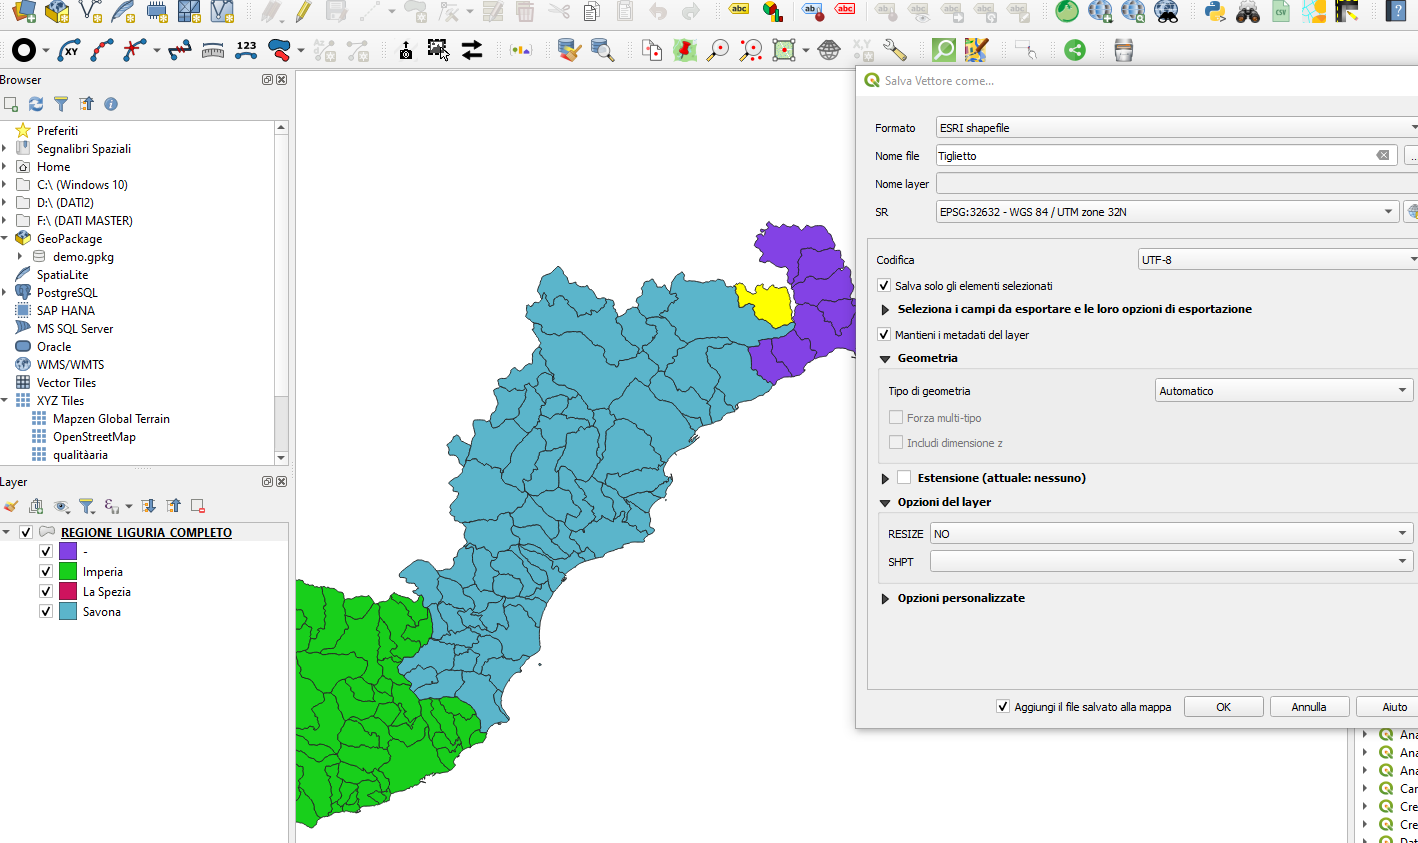
\includegraphics[width=0.75\linewidth]{tiglietto 3.png}
       
       \label{fig:enter-label}
   \end{figure}
\end{frame}




\begin{frame}
   \frametitle{Tabella Attributi, Modificare un record usando il calcolatore di campi e la selezione}
  
    \begin{itemize}
        \item Potremmo voler ribattezzare il Comune di Chiusavecchia in Chiusanuova
        \item Per Farlo da prima usiamo lo strumento selezione per espressione
        \item Poi utilizziamo il calcolatore di campi per aggiornare il dato
        \begin{figure}
            \centering
            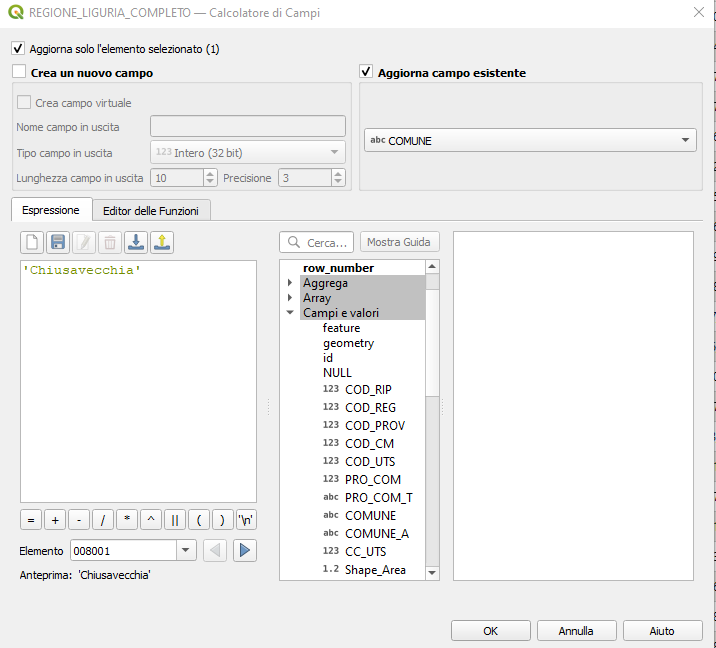
\includegraphics[width=0.5\linewidth]{chiusavecchia .png}
            
            
        \end{figure}
        \begin{figure}
            \centering
            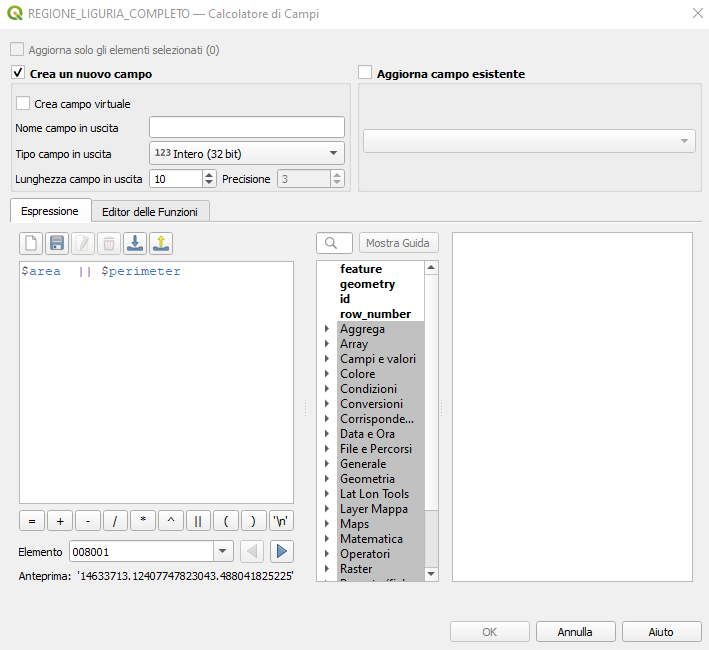
\includegraphics[width=0.60\linewidth]{areaperimetro.png}
            
            
        \end{figure}
    \end{itemize}    
   
\end{frame}

\section{Altri dati vettoriali}
 \begin{frame}
   \frametitle{I Dati vettoriali da CSV}
   \begin{itemize}
       \item I dati CSV sono dati la cui origine proviene da sistemi database,fogli di calcolo e similari. Tuttavia se importati in maniera corretta e con la presenza di coordinate, diventano veri e propri file vettoriali con relativa geometria
       \begin{figure}
           \centering
           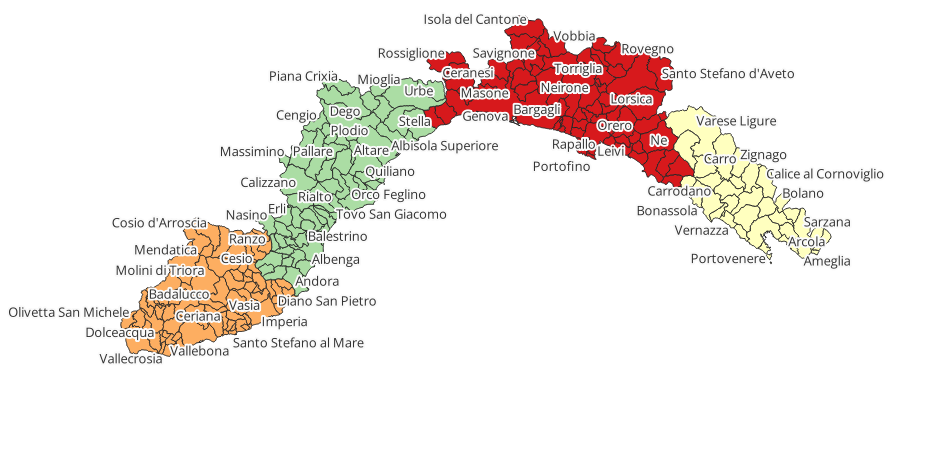
\includegraphics[width=0.75\linewidth]{immagine.png}
           
           \label{fig:enter-label}
       \end{figure}
   \end{itemize}
   \end{frame}

\begin{frame}
   \frametitle{I Dati vettoriali da CSV}
   \begin{itemize}
       \item Per usare i dati di origine CSV portarsi nel menù Layer selezionare aggiungi layer -> da testo delimitato
       \begin{figure}
           \centering
           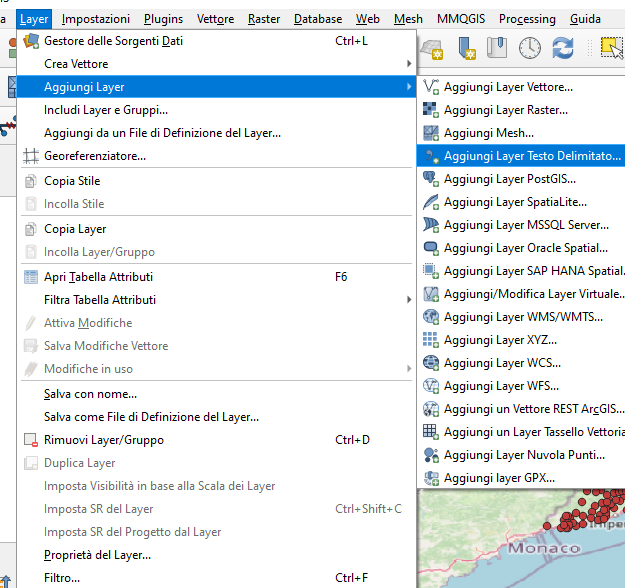
\includegraphics[width=0.5\linewidth]{layer.png}
                     
       \end{figure}
   \end{itemize}
   \end{frame}  

\begin{frame}
   \frametitle{I Dati vettoriali da CSV}
   \begin{itemize}
       \item Nella finestra di selezione del file teniamo conto di usare gli opportuni separatori del file csv, generalmente i file provienti da DB usano virgola ma potremmo avere altre situazioni, in ogni caso QGIS mostra un anteprima del file.
       \begin{figure}
           \centering
           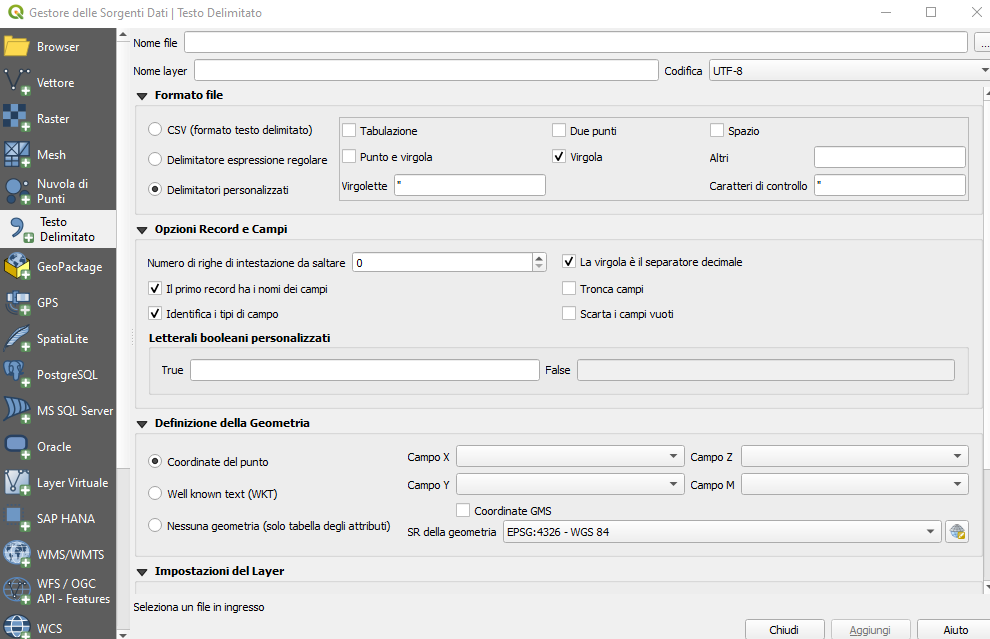
\includegraphics[width=0.5\linewidth]{layercsv.png}
        \item Se nel file csv che usiamo sono presenti Latitudine e Longitudine oppure X e Y dobbiamo indicare all'interfaccia tali campi, e indicare il sistema di Riferimento eventualmente
        
           
       \end{figure}
   \end{itemize}
   \end{frame}  




\section{Simbologia}
\subsection{Simbologia e rappresentazione del dato}

\begin{frame}{Simbologia e rappresentazione del dato}
    \begin{center}
        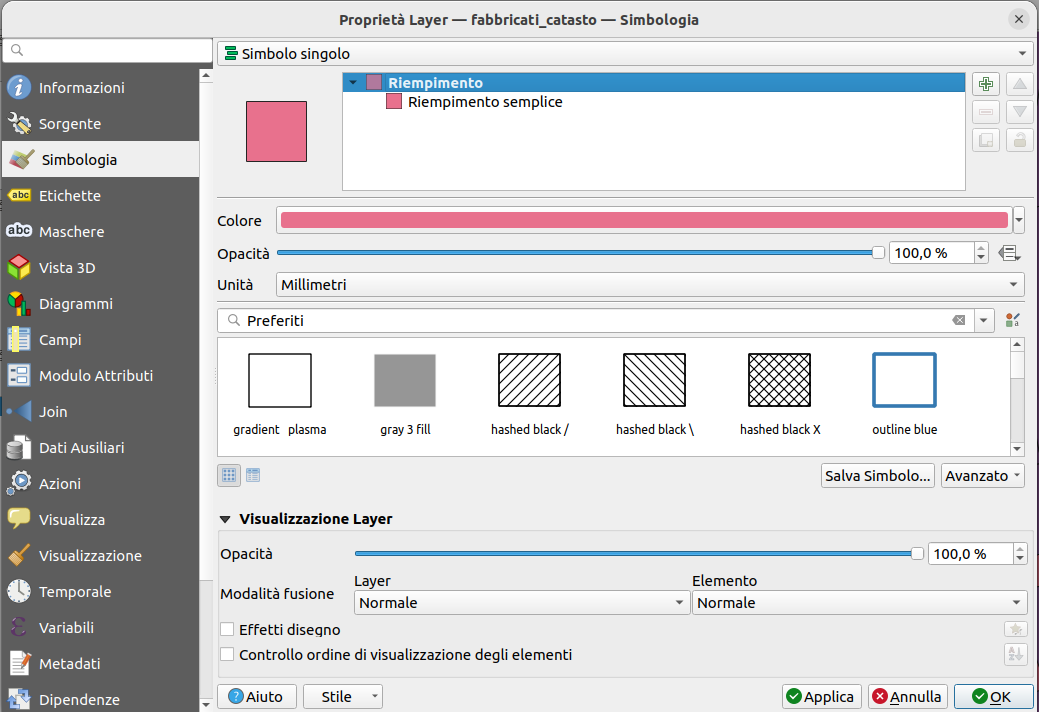
\includegraphics[width=.95\textwidth]{digitizing_pics/SImbologia del 2022-10-12 10-05-05.png}
    \end{center}
\end{frame}

\begin{frame}{Simbologia e rappresentazione del dato}
    La rappresentazione del dato ha un ruolo molto importante nella comunicazione del significato stesso che il dato porta con sé, pensiamo a come rappresenteremmo per esempio:
    \begin{itemize}
        \item aree verdi
        \item aree contaminate
        \item zone pedonali
        \item cartelli stradali
        \item ...
    \end{itemize}

    La simbologia non fa parte però delle caratteristiche o degli attributi del dato stesso, sono piuttosto attributi del progetto QGIS e sono condivisi solo concedendo l'accesso al progetto stesso.
\end{frame}

\begin{frame}{Etichettatura e Stili}
\begin{figure}
    \centering
    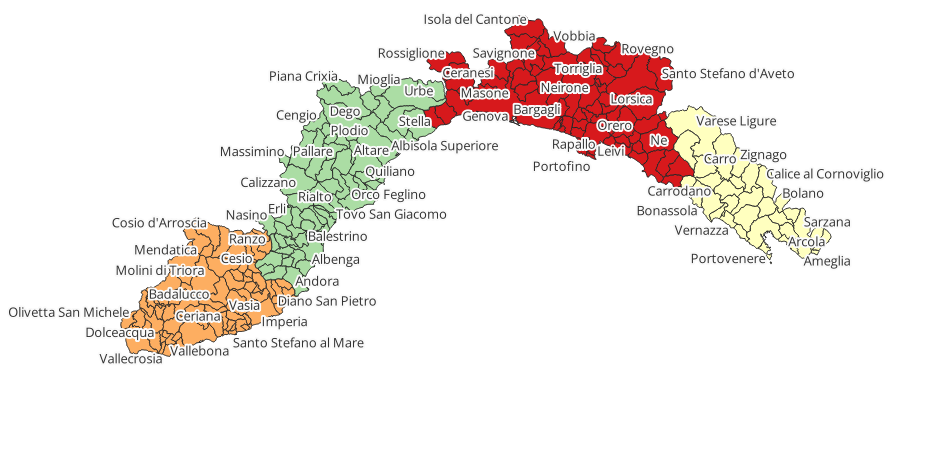
\includegraphics[width=1\linewidth]{immagine.png}
   
    
    
\end{figure}
    
\end{frame}

\begin{frame}{Etichettatura}
\begin{figure}
   
        \centering
        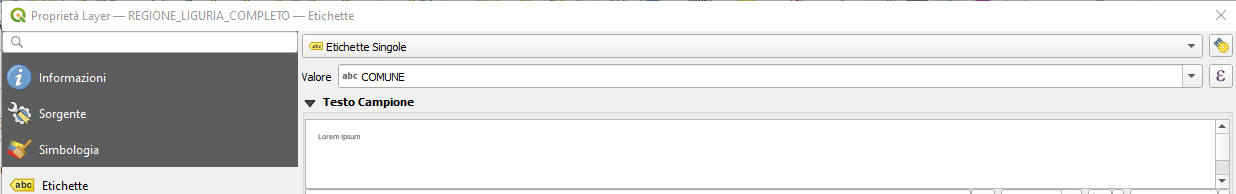
\includegraphics[width=1\linewidth]{etichette.png}
        \begin{itemize}
            \item per applicare l'etichettatura degli elementi vettoriali, bisogna usare il tasto del destro del mouse sul vettore a cui applicare etichette.
            \item le etichette provengono dai campi della tabella attributi        
        \end{itemize}
        
        
    \end{figure}
    
\end{frame}

\begin{frame}{Simbologia}
\begin{figure}
     \centering
     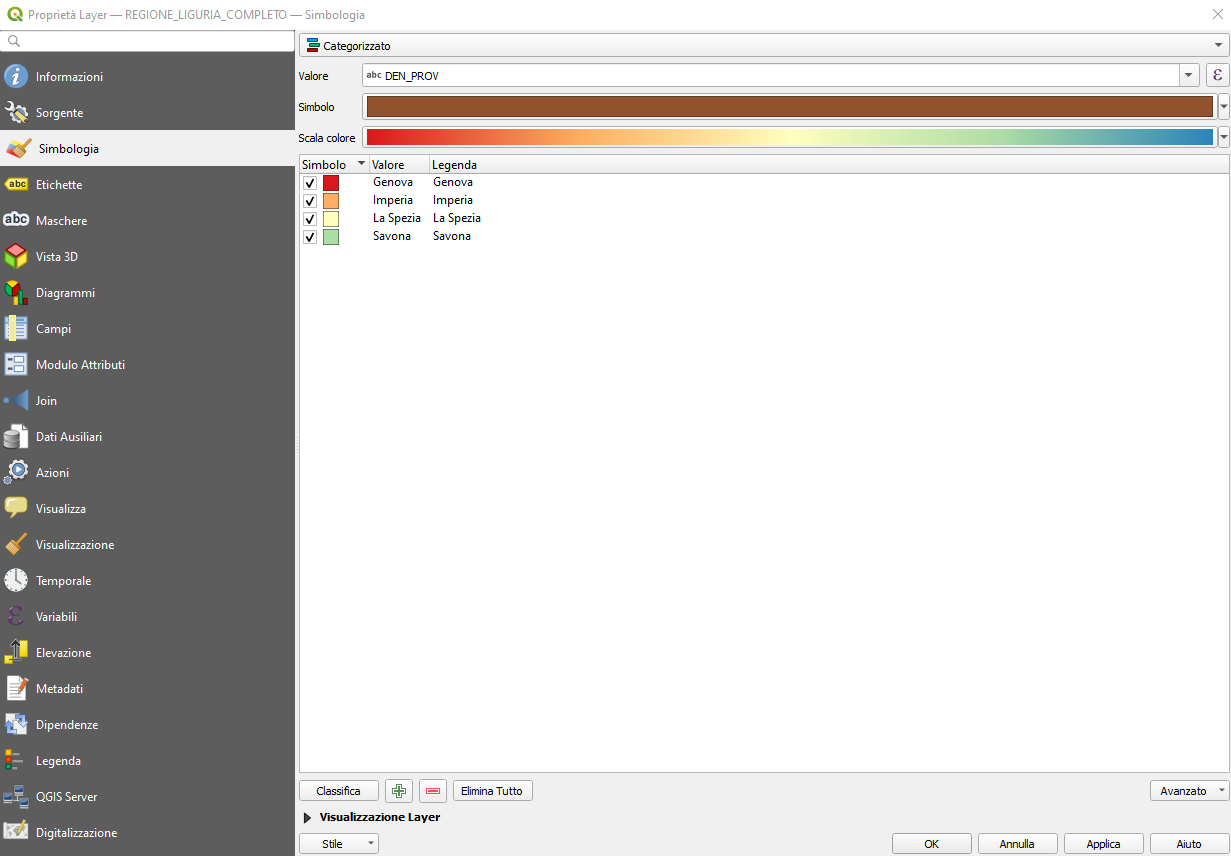
\includegraphics[width=0.75\linewidth]{corso2023/simbologia.png}
     
 \end{figure} 
    
\end{frame}

\begin{frame}{Stili multipli e Temi}
    Il pulsante a discesa "Gestisci Viste Mappa" fornisce l’accesso a comode scorciatoie per manipolare la visibilità dei layer nella Tabella dei Contenuti:
    \begin{figure}
         \centering
         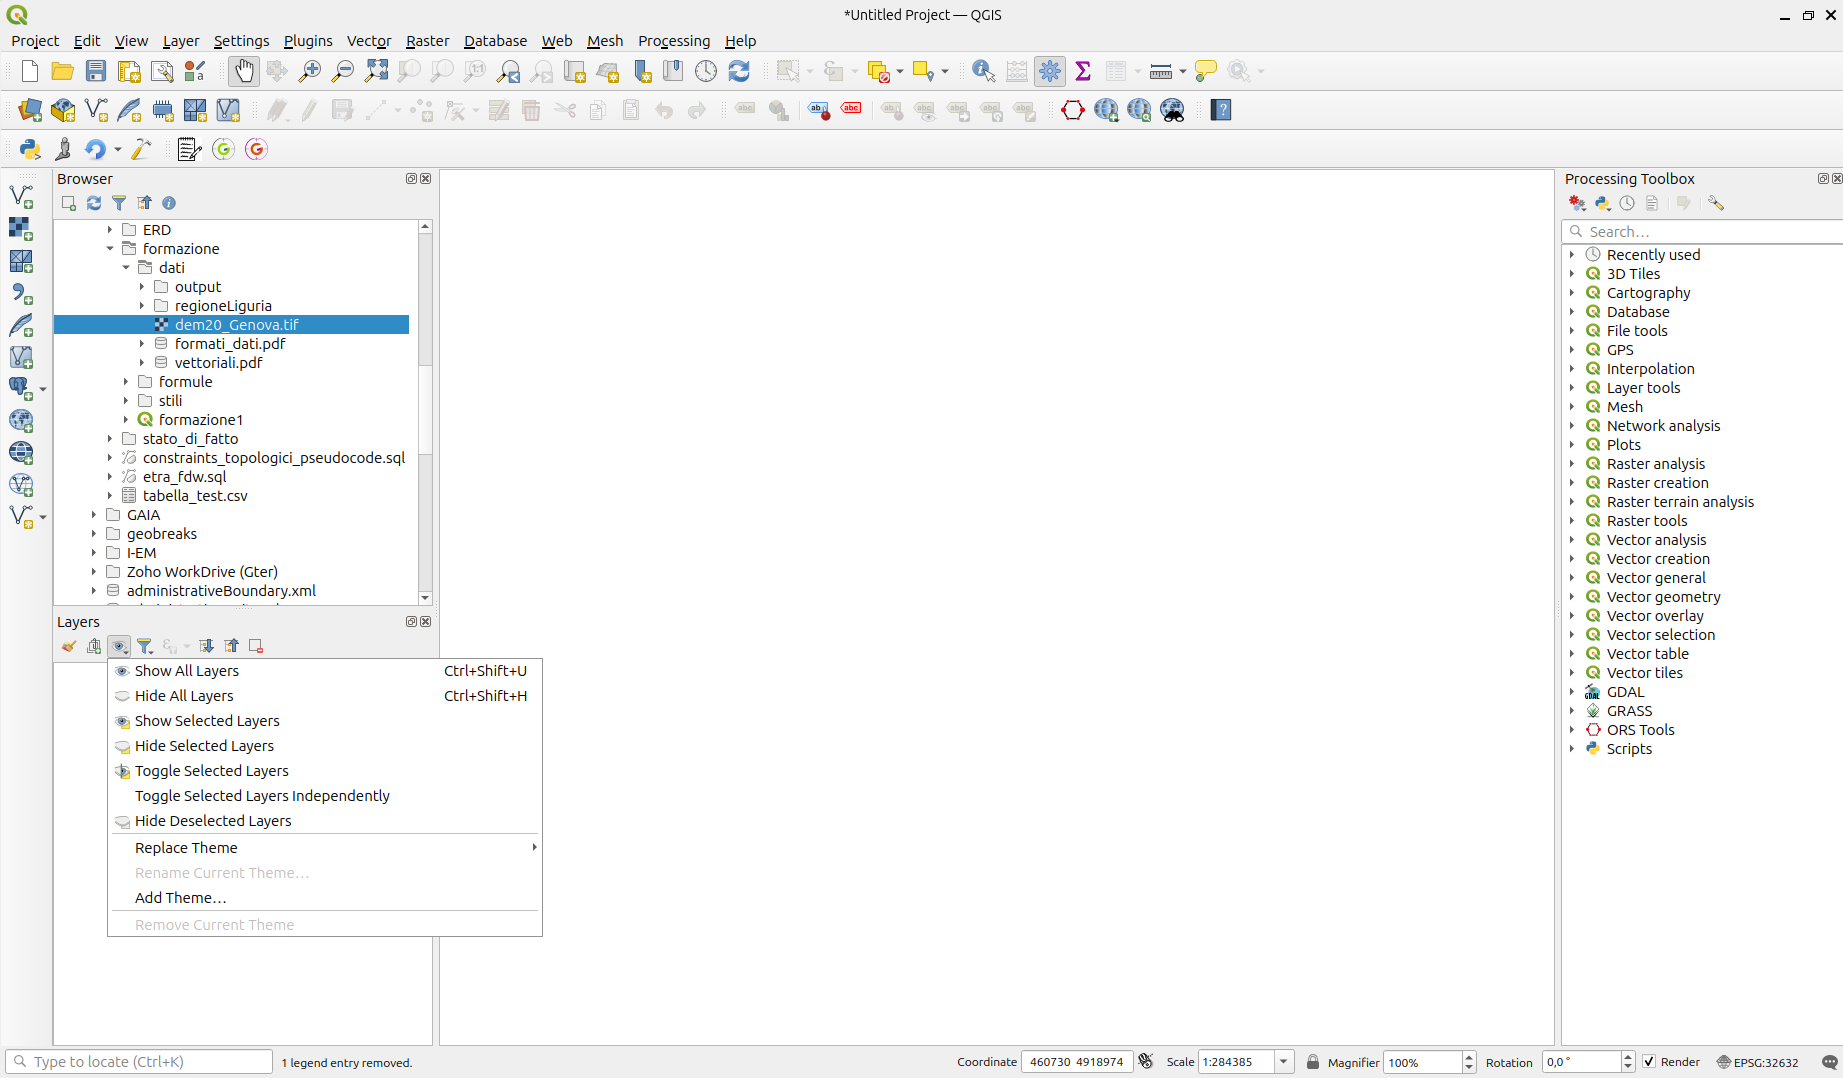
\includegraphics[width=0.75\linewidth]{digitizing_pics/stili_multipli_1.png}
     
    \end{figure} 
\end{frame}

\begin{frame}{Stili multipli e Temi}
    Ma oltre al semplice controllo della visibilità dei layer, è possibile anche configurare viste mappa nella legenda, e passare da una vista ad un'altra, permettendo una gestione avanzata della visualizzazione layer.

    Una vista mappa altro non è che uno "screenshot" della legenda della mappa corrente, che compende:
    \begin{itemize}
            \item Il riferimento allo stile del layer
            \item Gli oggetti impostati come visibili o non visibili
            \item lo stato (collassato o espanso) dei group layers e dei sottogruppi al suo interno
    \end{itemize}

\end{frame}

\begin{frame}{Stili multipli e Temi}
    Per creare una nuova Vista Mappa:
    \begin{itemize}
            \item Seleziona un layer che vuoi venga mostrato
            \item Configura le proprietà del layer (simbologia, diagramma, etichette…..) come visto in precedenza
            \item Espandi il menu \textbf{Stile} $\rightarrow$  \textbf{Aggiungi} e memorizza le impostazioni come a \textbf{new style embedded in the project}.
    \end{itemize}
\end{frame}

\begin{frame}{Stili multipli e Temi}
    
    \begin{figure}
         \centering
         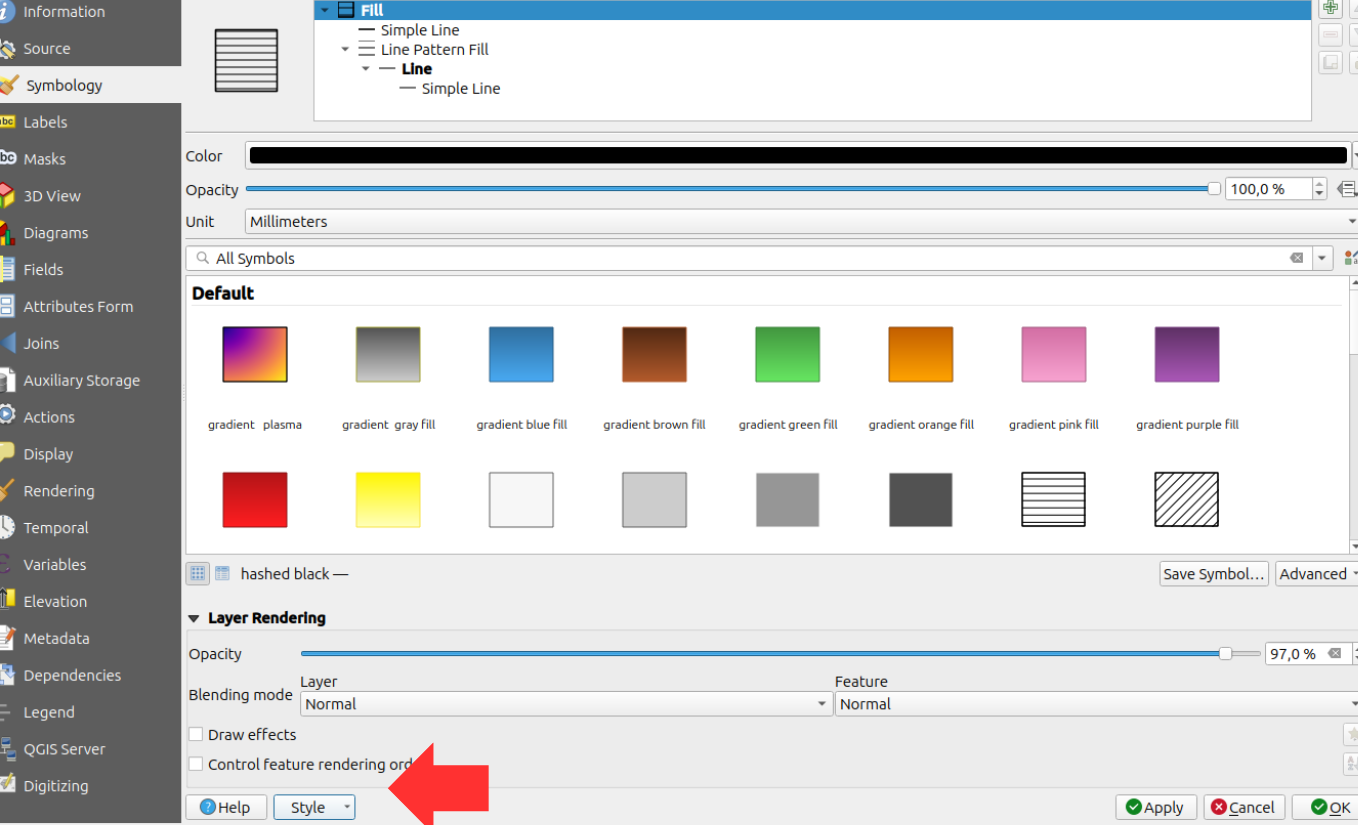
\includegraphics[width=0.75\linewidth]{digitizing_pics/stili_multipli_2.png}
     
    \end{figure} 
\end{frame}



}
\subsection{Contatti e licenze}
{
\setbeamertemplate{footline}{} 
\setbeamertemplate{headine}{} 
\frame{	
\addtocounter{framenumber}{-1}  % non conto questa slide
\begin{center}
\bigskip

\includegraphics[width=0.2\textwidth]{./Gter.png} \\ 
\scriptsize{
%Gter srl Innovazione in Geomatica Gnss e Gis\\

Via Jacopo Ruffini 9/1A\\
16128, Genova \\
formazione@gter.it\\}
\normalsize
\bigskip
\href{www.gter.it}{\textcolor{gter}{\emph{www.gter.it}}}
	
\bigskip	

  	\href{https://twitter.com/@gteronline} { 
\includegraphics[width=0.15\textwidth]{./tw.jpg}}
	\hspace{30pt}
	 \href{http://www.facebook.com/Gteronline} { 
\includegraphics[width=0.15\textwidth]{./fb.jpg}}
		\hspace{30pt}
%	 \href{ https://plus.google.com/+GterIt/posts} { \includegraphics[width=0.15\textwidth]{../go.png}}
%	 \hspace{30pt}
	 \href{http://www.linkedin.com/company/gter-srl-innovazione-in-geomatica-gnss-e-gis} { 
\includegraphics[width=0.15\textwidth]{./ln.png}}
	 
	 
	 

	 
\bigskip
\vspace{30pt}

	
	\href{http://creativecommons.org/licenses/by-sa/3.0/deed.it} {	
	
\includegraphics[width=0.15\textwidth]{./88x31.png} 
	\\	
	\tiny Quest' opera è distribuita con licenza Creative Commons Attribuzione - Condividi allo stesso modo 3.0 Unported.} 	
	
	
	
\end{center}
%\tableofcontents[pausesections,part=2]
}
}

\end{document}
